\documentclass[letterpaper,journal]{IEEEtran}
\usepackage{amsmath,amssymb}
\usepackage{graphicx}
\usepackage{booktabs,array,tabularx}
\usepackage{cite}
\usepackage{url}
\usepackage{stfloats}
\usepackage[hidelinks]{hyperref}
\hypersetup{pdftitle={Beyond Sampling Rate: Reference-Based Energy Measurement Across Edge-AI Platforms},
pdfauthor={Kevin Mika, Joris Wachsmuth, Florian Porrmann, Jens Hagemeyer},
pdfsubject={IEEE TIM working manuscript v0.3, 9 October 2026}}
\graphicspath{{figures/}}
\newcommand{\urecs}{u.RECS}
\newcolumntype{Y}{>{\raggedright\arraybackslash}X}
\renewcommand{\dbltopfraction}{0.9}
\renewcommand{\textfraction}{0.06}
\setcounter{dbltopnumber}{2}
\hyphenation{mea-sure-ment re-con-struc-tion ac-cel-er-a-tor}
% Generated from frozen exported observations.
\newcommand{\PauseReduction}{8.7}
\newcommand{\HailoLLMCV}{46.1}
\newcommand{\HailoLLMShift}{24.3}
\newcommand{\VariableEnergyFive}{-10.3}
\newcommand{\VariablePowerFive}{-0.7}
\newcommand{\VariableSpanFive}{-9.7}
\newcommand{\FPFifty}{0.63}

\begin{document}
\title{Beyond Sampling Rate: Reference-Based Energy Measurement Across Edge-AI Platforms}
\author{Kevin Mika, Joris Wachsmuth, Florian Porrmann, and Jens Hagemeyer%
\thanks{The authors are with CITEC, Bielefeld University, Inspiration 1, 33619 Bielefeld, Germany. Corresponding author: Kevin Mika (e-mail: kmika@techfak.uni-bielefeld.de).}%
\thanks{Working journal manuscript v0.3, 9 October 2026. Prepared for development toward IEEE Transactions on Instrumentation and Measurement; not submitted.}}
\markboth{IEEE TIM Working Manuscript, October 2026}{Mika et al.: Reference-Based Energy Measurement Across Edge-AI Platforms}
\maketitle
\begin{abstract}
Energy measurement for edge inference requires a sampling rate suited to the intended quantity, a defined electrical boundary and a representative execution interval. We develop and evaluate a reference-based workflow that separates numerical sampling error, recorded power fluctuations and deployed measurement behaviour on Jetson and Hailo. Across six Jetson workloads and 59 paired executions, native-trace reconstruction at 2 kS/s meets an empirical hierarchical 1\% energy-error criterion at the tested 2-, 5- and 10-s intervals; a 100-ms interval instead requires a persistent 80-kS/s minimum on the tested grid. A separate 104-s FP16 study passes its pooled energy criterion at 50 S/s, whereas the evaluated 125/160-kS/s rates meet its 95/99\% measured-variance coverage targets. The deployed comparisons show why those rate decisions are only a starting point. Embedded/external median power differences remain below 0.5\% for continuous Jetson operation and the three Hailo workloads at 300 s, but variable Jetson activity gives 2.9\%. For variable Hailo activity at a 5-s request, telemetry mean-power disagreement is only $\VariablePowerFive\%$ while energy disagreement is $\VariableEnergyFive\%$, with different retained intervals. Spectral comparisons and controlled execution tests identify further acquisition and protocol dependencies. The resulting approach validates the measurement configuration as a whole rather than prescribing a universal sampling rate or ranking meters across different electrical boundaries.
\end{abstract}
\begin{IEEEkeywords}
Energy measurement, instrumentation, edge AI, sampling rate, measurement boundary, power spectral density, accelerator telemetry.
\end{IEEEkeywords}
\section{Introduction}
\IEEEPARstart{E}{nergy} benchmarking usually ends with a simple quantity: joules consumed by an execution, or the mean power needed to sustain it. Obtaining a trustworthy number requires several decisions that are less simple. A meter must observe the intended electrical boundary, cover the intended execution interval and represent the signal at an adequate rate. Repeating the experiment should also reproduce the work and operating conditions. A precise answer to only one of these questions can leave the final comparison misleading.

Consider an embedded power sensor, vendor telemetry and a plug-level AC meter. All three may produce stable readings during the same benchmark, yet they need not describe the same quantity. A Jetson module combines processing and supporting circuitry behind its DC input. A Hailo M.2 card performs inference with assistance from a separate host, which the card-input measurement excludes. A meter at the supply input adds conversion and any other connected loads. Agreement between these observations is therefore conditional on more than their nominal sampling rates.

The integration interval creates a second, independent difficulty. Two streams can report nearly the same average power while covering different parts of an execution. Their energies will then differ even before considering sensor calibration. Conversely, a low-rate trace can reproduce a long energy integral while missing most of the recorded power fluctuations. These are not contradictory results; they answer different measurement questions.

Our approach is to make those questions explicit and test them separately. High-rate recordings establish how a sampled representation changes an integral over fixed endpoints. Spectral analysis characterises the recorded fluctuations that an energy integral can average away. Physical repetitions then test the actual acquisition procedure, including interval selection, execution order and starting state. This sequence connects measurement validation to the settings used in a deployed benchmark rather than treating the oscilloscope result as a universal prescription.


The experimental study combines an integrated Jetson platform with a Hailo-10 M.2 accelerator. Jetson provides the controlled foundation: paired high-rate recordings quantify rate--duration decisions, and a separate long-window study tests whether energy agreement implies preserved fluctuations. Deployed PicoScope, \urecs{}, telemetry and scaled Shelly observations then test those decisions within each platform's recorded executions. The Hailo card-input study broadens the analysis to an attached accelerator with a different boundary and workload dynamics. We compare measurement procedures, not accelerator efficiency; the records do not establish identical compiled workloads across platforms.

Four research questions organise the complete measurement argument:
\begin{enumerate}
\item[\textbf{RQ1:}] Which tested sampling rates preserve interval energy, and how does the required rate change with the integration duration?
\item[\textbf{RQ2:}] How do energy-preserving rates differ from those needed to describe measured fluctuations, and how does the acquisition path affect that description?
\item[\textbf{RQ3:}] How does agreement between deployed measurement paths depend on the electrical boundary, workload and actual integration interval?
\item[\textbf{RQ4:}] How do execution duration and starting conditions affect the representativeness of repeated measurements after the rate has been chosen?
\end{enumerate}

The findings follow this sequence. Fixed-endpoint reconstruction identifies when low-rate energy integration is adequate. The same energy agreement can coexist with poor coverage of recorded fluctuations. Physical meter comparisons then expose a different issue: nearly equal mean powers can yield different energies when intervals or electrical domains differ. Finally, balanced acquisition and fixed-rate pause tests establish why execution conditions must be checked alongside the observation itself. Each step addresses a limitation that the preceding step cannot resolve alone.

This article extends our Jetson-focused study \emph{How Fast Is Fast Enough?}~\cite{mika2026workshopdraft}. Its measurement framework and central Jetson findings are presented here as the foundation of a self-contained journal account, not as newly obtained results. The additional experimental content comprises Hailo card-input and spectral measurements, duration-wise joint comparisons of energy, power and interval span, and a separate fixed-rate pause diagnostic. The instrumentation and initial validation also build on Wachsmuth's thesis~\cite{wachsmuth2026thesis}. The extension therefore broadens the measurement evidence while keeping its underlying quantities and validation logic explicit.

\section{Related Work}
\subsection{Comparable Work Is Only One Part of a Comparable Measurement}
Benchmarking frameworks establish what a system is asked to execute and how performance and energy should be reported. MLPerf Tiny and MLPerf Power address widely different operating scales, while MLPerf Inference specifies power-measurement procedures~\cite{banbury2021mlperftiny,tschand2024mlperfpower,mlcommonsInferencePower}. Edge studies apply such measurements to specialised platforms and deployment choices~\cite{liang2020,baller2021,libutti2020usbaccelerators}. These efforts make experimental work more comparable. They do not make a module-input observation, a card-input observation and a supply-input observation interchangeable. Our concern is the measurement decision that precedes interpreting their numbers: which quantity and interval does a particular acquisition actually support?

\subsection{Calibration and Temporal Resolution Answer Different Questions}
External instruments provide a way to test internal readings. Shalavi et al. use externally referenced regression to calibrate built-in sensors on several Jetson devices~\cite{shalavi2023jetsoncalibration}. PowerSensor3 provides open measurement hardware and software for direct power acquisition~\cite{vanderVlugt2025powersensor3}. These approaches address the reliability and accessibility of the observation. A further test is needed when the desired output changes from a long average to a short event: agreement in level does not establish sufficient temporal detail.

The closest methodological connection is Gralka et al.'s \emph{Power Overwhelming}~\cite{gralka2024poweroverwhelming}. It combines oscilloscope measurements, external instruments and vendor interfaces, with synchronisation to rendering activity. Its comparison of aggregate readings and within-frame structure demonstrates why one instrument can be useful for energy totals yet inadequate for detailed activity analysis. We build on that distinction rather than treating the combination of meters as new. Our focus is the joint interpretation of finite-interval reconstruction, recorded spectral coverage and practical measurement boundaries in edge-AI inference.

\subsection{Telemetry Polling Is Not Physical Sampling}
Software-accessible power data introduce update and averaging behaviour in addition to electrical response. Evaluations of Jetson sensors, RAPL counters and software-based meters show why the interface and reported domain belong in the measurement description~\cite{aslan2022jetsonbuiltin,alt2024raplheteromemory,jay2023softwarepowermeters}. Yang et al. examine NVIDIA sensor behaviour across GPU generations, motivating device-specific rather than universal assumptions about built-in telemetry~\cite{yang2024parttime}.

Dauner et al. study how the polling interval affects RAPL and NVML energy readings, including comparisons with external instruments~\cite{dauner2026frequency}. Their results concern the interaction of counters, stale readings and acquisition overhead. Our same-trace experiment changes a numerical grid after the physical execution has finished; our deployed-meter experiment instead preserves each path's recorded intervals and response. Keeping these experiments separate avoids explaining every difference between physical acquisitions as a sampling-grid effect.

Together, this literature motivates a hierarchy of checks, not a single winning meter. Calibration addresses the level, reconstruction tests a defined integral, spectral analysis describes observed dynamics, and physical repetitions test the deployed procedure. The present study connects these checks through Jetson and Hailo observations. Its duration-wise pairing adds a practical distinction between agreement in mean power and agreement in integrated energy without claiming a synchronised, event-level telemetry calibration.

\section{Measurement Design}
\label{sec:design}
\subsection{Define the Quantity Before Comparing the Instruments}
For a stated electrical boundary and interval $[t_0,t_1]$, we report delivered energy and mean power as
\begin{equation}
E=\int_{t_0}^{t_1}U(t)I(t)\,\mathrm{d}t,
\qquad \overline P=\frac{E}{T},\quad T=t_1-t_0.
\label{eq:quantity}
\end{equation}
The benchmark duration request controls the execution command; it is not substituted for $T$. This distinction is essential for short runs and for intervals containing pauses or padding. Recorded power is integrated with the trapezoidal rule using its timestamps or documented sample interval.

Figure~\ref{fig:boundaries} separates the observed electrical domains. The Jetson measurement is at the DC input associated with the \urecs{}-mounted module. The Hailo measurement covers the complete M.2 card input, not the host that supplies data and schedules inference. Shelly observes the connected AC supply arrangement. This includes conversion and any auxiliaries powered inside that arrangement; it does not establish that every host component is included. Vendor telemetry retains the domain reported by its interface. The AC/DC difference consequently cannot be assigned directly to host energy or to an intrinsic meter error.

\begin{figure*}[t]
\centering
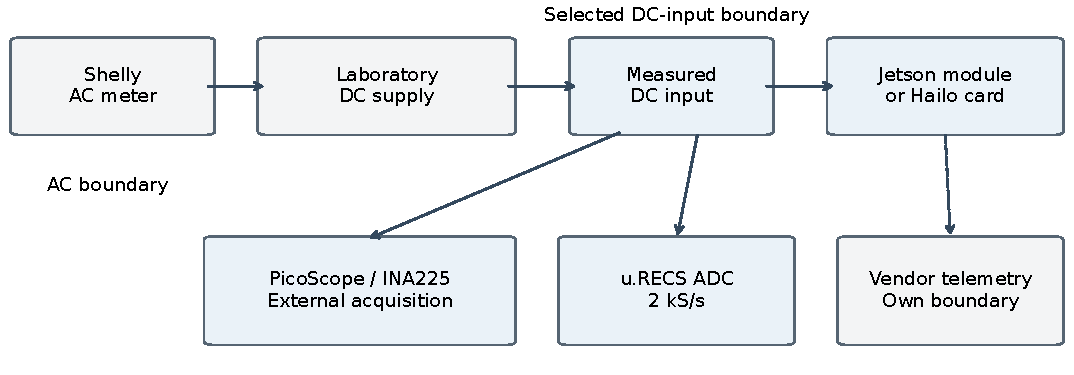
\includegraphics[width=.92\textwidth]{measurement_boundaries.pdf}
\caption{Observation boundaries in the Jetson and Hailo experiments. External DC acquisition and embedded sensing address the selected module/card input; telemetry retains its reported domain and Shelly the connected AC supply boundary. The Hailo card observation excludes its host. This diagram is not a measured host/card energy decomposition.}
\label{fig:boundaries}
\end{figure*}

\subsection{Acquisition Paths and Their Validation}
The Jetson platform is an Orin NX 16 GB mounted on \urecs{}~\cite{recs2026,wachsmuth2026thesis}. Its documented direct-study configuration uses a nominal 19-V supply, JetPack 6.2.1 / Linux for Tegra 36.4.7 and fixed maximum clocks. These settings describe that study, not an assumed configuration of every control or waveform recording. Hailo-10 measurements use the separately observed M.2 card and the workload deployments recorded with each experiment.

The external DC setup uses a 20-m$\Omega$ shunt, INA225 amplifier and PicoScope 4224A, streaming at up to 5 MS/s. Its nominal differential current-path bandwidth is approximately 77 kHz; the voltage-input bandwidth is 20 MHz. \urecs{} uses a nominally equivalent analogue path with an ADS7953 12-bit ADC at 2 kS/s. Jetson INA3221, HailoRT and the approximately 1-S/s Shelly Plus Plug S provide additional observations. The paired-scope study adds a Tektronix TCP0030A current-probe acquisition path and retains each path's recorded calibration and voltage treatment~\cite{energyResults2026}.

The current paths were calibrated against an EA-EL 9080-60 DT electronic load and Fluke 179 reference, using endpoint gain and offset followed by a separate verification sweep~\cite{wachsmuth2026thesis}. The sweep covers 36 settings over 0--3.5 A using ten-second means. Across the nonzero settings, maximum absolute relative current deviations are about 2.0\% for PicoScope/INA225 and 0.44\% for \urecs{}. This verifies the static correction under the tested conditions. Dynamic power uncertainty is a different question, because bandwidth, timing and voltage treatment remain in the measurement chain.

For paired-scope power, the documented current-dependent voltage model gives $\widehat P=I(a+bI)$ over a characterised 0--3.5-A range. Currents outside that range are extrapolated rather than clipped. YOLO-FP32 alone retains a workload-derived Tektronix offset correction; its dependence on the comparison path limits independent absolute-agreement claims. Other studies retain their recorded voltage measurements or estimates. In particular, the Jetson embedded path and Shelly comparisons retain setup-derived scaling, rather than being refitted to improve agreement here. Full coefficients, verification data and transformation order are in the source package~\cite{energyResults2026}.

These checks have distinct roles. The static verification tests gain and offset after calibration; it does not establish the temporal fidelity of the complete power path. Faster Tektronix observations provide a separate spectral check: at 250 MS/s, the largest reported variance fraction above the 2.5-MHz Nyquist limit of a 5-MS/s recording is about 0.015\% across the six workloads. GEMM-FP32 uses active-only variance in this check, while the other workloads use active-minus-idle variance. This supports the chosen high-rate observation for these signals without treating a small spectral tail as an absolute power-accuracy bound~\cite{energyResults2026}.


\subsection{Complementary Experiments, Not One Pooled Dataset}
The experiments separate questions that cannot be answered by one set of repeats (Table~\ref{tab:cohorts}). The same-trace study contains ten paired executions each for GEMM-FP32, GEMM-INT8, YOLO-FP32, YOLO-INT8 and Gemma3-4B, and nine for ResNet-50 FP32: 59 executions observed through two paths. The FP16 illustration is a separate set of 15 long recordings with nominal 104-s energy intervals. Hailo spectral results use 15 GEMM and 15 YOLO recordings. These waveform studies are not counted as additional repeats of the duration or direct-rate studies.

\begin{table*}[t]
\caption{Experimental roles and physical units. Numerical offsets, multiple sensor observations and reused summaries are not additional independent executions. Detailed per-series identities and eligibility counts accompany the results.}
\label{tab:cohorts}
\centering\small
\begin{tabularx}{\textwidth}{@{}p{.22\textwidth}p{.32\textwidth}Y@{}}
\toprule
Question & Observations & What is held fixed or compared \\
\midrule
Energy reconstruction & Six Jetson workloads: 59 Tek/Pico pairs; separate FP16: 15 recordings & Same recorded execution and endpoints; target grids vary \\
Measured fluctuations & Native paired-scope spectra; 30 Hailo GEMM/YOLO recordings; FP16 active/idle segments & Active and idle descriptions retain their acquisition response \\
Duration and deployed meters & Seven Jetson and three Hailo series; ten requests from 5 to 600 s & Recorded executions are paired within series; 150 executions at 300 s yield 450 comparator pairs \\
Direct acquisition repeatability & Eight Jetson and four Hailo rate series; 323 groups, 4842 finite results & Different physical executions at configured rates \\
Protocol controls & Twelve FP16 rate-order runs; six scored FP32 pause runs & Fixed completed queries; complementary rates or changed process pauses \\
\bottomrule
\end{tabularx}
\end{table*}

The direct studies include continuous GEMM and YOLO, variable YOLO activity and an LLM-labelled series. The Jetson direct LLM is Gemma3-12B; the paired-scope Gemma3-4B is a different workload. For Hailo, the retained model labels do not establish every compiled-model, input, batch or runtime parameter. They identify within-series measurement comparisons, not semantically matched cross-platform efficiency tests. No common inference count, missing precision or host share is inferred from a shared workload name.

The direct-rate grid normally has 27 configured rates and 15 repetitions per rate; Jetson YOLO-FP32 has 26 rate groups. All finite results remain in the selected series. Three Hailo-LLM executions lack a valid load interval and are not replaced by zeros. The duration study has 450 finite Hailo and 1022 finite Jetson load results. Each of its 300-s meter comparisons contains all 15 paired executions per workload; shorter-duration groups retain their actual available counts.

\section{Analysis: Separate the Sources of Disagreement}
\label{sec:methods}
\subsection{An Operational Interval That Retains Internal Pauses}
Direct acquisition begins before the benchmark and ends after it, so the analysis needs an explicit load interval. We use time-weighted 100-ms power bins, recording-edge medians for the baseline and the 95th percentile for the active level. A load must exceed both a relative contrast criterion and a robust edge-variation criterion. The main detector requires at least 200 ms above the midpoint between baseline and active level, then retains the envelope from the first to the last qualifying segment. Internal pauses remain part of that interval.

This rule defines the measured quantity; it does not create hardware-synchronised inference markers. Thresholds at 0.4 and 0.6 of the contrast provide sensitivity checks around the main 0.5 rule. An interval is not chosen to fit the requested runtime or to minimise a measurement difference. Hailo variable YOLO retains its explicitly recorded interval, including padding, because a sustained high starting level does not supply a reliable detected onset. This same rule is retained across its rate and duration comparisons. The interval policy and full detector conditions are recorded with the exported results~\cite{energyResults2026}.

\subsection{Pair Energy, Mean Power and Span Before Aggregation}
For each series, comparator $s$ and requested duration, we intersect the recorded execution IDs with PicoScope IDs. For $X\in\{E,\overline P,T\}$, the signed pair difference is
\begin{equation}
\delta_{X,r}=100\left(\frac{X_{s,r}}{X_{\mathrm{Pico},r}}-1\right).
\label{eq:paired}
\end{equation}
The reported central value is the median of these individual differences. It is not a ratio of two group medians. Empirical fifth and 95th percentiles describe repeat spread and remain available in the numerical artefact; they are not confidence intervals or absolute calibration uncertainties.

Comparing all three quantities prevents an important ambiguity. For each pair, their ratios satisfy
\begin{equation}
\frac{E_{s,r}}{E_{\mathrm{Pico},r}}=
\frac{\overline P_{s,r}}{\overline P_{\mathrm{Pico},r}}
\frac{T_{s,r}}{T_{\mathrm{Pico},r}}.
\label{eq:identity}
\end{equation}
Thus, close mean-power agreement need not imply close energy agreement. Equation~\eqref{eq:identity} holds for the individual pair; multiplying separately reported group medians is not an exact decomposition. The original intervals and voltage transformations remain unchanged throughout. Pairing identifies the same execution, not necessarily the same physical endpoints or electrical domain.

Duration curves use each run's $E/T$, normalised to its workload's median in the 600-s-request group. This is a within-series reference, not an assumed steady-state limit. Direct-rate repeatability uses the population energy standard deviation divided by its mean. The displacement of a rate group compares its mean with the equally weighted mean of all rate-group means. This consistent mean-based statistic describes differences between physical executions, not an isolated numerical integration error.


\subsection{Use Fixed Endpoints to Test the Sampling Representation}
\label{sec:reconstruction-method}
A direct acquisition-rate sweep changes more than a vector's sample spacing: each point belongs to another physical execution. To isolate the numerical representation, we instead reconstruct interval energy from a single high-rate recording. That recording supplies both the reference integral and all candidate grids. The executed workload, analogue response, voltage treatment and integration endpoints therefore remain fixed while the target rate and grid offset change.

Let $P_{\mathrm{ref}}(t)$ be the calibrated native 5-MS/s power representation over a selected interval of duration $T$. Its integral gives $E_{\mathrm{ref}}$. At target rate $f$, the sample grid is shifted within one target period by an offset $0\leq\delta<1/f$. The offset concerns when the power signal is sampled, not the phase between a voltage and current channel. The reconstruction samples the reference representation on that grid, retains the source endpoint values and integrates the resulting piecewise-linear power representation. No additional target-rate anti-alias filter is applied in the primary comparison.

The absolute relative energy error is
\begin{equation}
e(f,T,\delta)=\frac{|\widehat E(f,T,\delta)-E_{\mathrm{ref}}|}{E_{\mathrm{ref}}},
\qquad E_{\mathrm{ref}}>0.
\label{eq:reconstruction-error}
\end{equation}
An error of zero would mean agreement with that recorded reference, not proof that the reference itself is an exact electrical truth. The experiment also does not reproduce every hardware behaviour of a lower-rate ADC: it isolates the consequences of changing the grid on already derived power. Calibration, voltage modelling and acquisition response remain part of the source trace.

The fixed test grid contains nine nominal durations, from 20 ms to 10 s, and 19 rates from 50 S/s to 160 kS/s. For each duration, up to 16 distributed windows test different portions of the recording; 64 offsets test alignment within a target period. An eligible case requires at least four target-grid samples. The full-duration case has one available span of 9.999999 s, rather than 16 independent ten-second recordings. Window and phase counts describe numerical cases, not physical repeats.

For path $m$, workload $w$, recording $r$, window $j$ and offset $k$, the empirical envelope is
\begin{equation}
q(f,T)=\max_{m,w}Q_{0.95,r}
\left[Q_{0.95,j,k}\left(e_{m,w,r,j,k}(f,T)\right)\right].
\label{eq:hierarchy}
\end{equation}
The inner percentile summarises the grid and window cases within one recording. The outer percentile then summarises recordings of that workload and measurement path. Finally, the maximum covers the twelve workload/path groups. This ordering prevents a recording with many derived windows from being interpreted as many independent executions. Percentiles use linear interpolation; the resulting envelope is an empirical criterion on these cohorts, not a confidence guarantee for future workloads.

A proposed fixed rate passes a tolerance $\varepsilon$ when $q(f,T)\leq\varepsilon$. A persistent minimum asks a stricter question: starting at which tested rate do \emph{all higher eligible tested rates} also pass? On the finite eligible rate set $\mathcal F_T$, it is
\begin{equation}
f_{\min,E}(T,\varepsilon)=\min\left\{f\in\mathcal F_T:
\max_{g\in\mathcal F_T,\,g\geq f}q(g,T)\leq\varepsilon\right\}.
\label{eq:persistent}
\end{equation}
If this set is empty, the criterion is not attained within the tested grid. No interpolation creates an untested threshold. Keeping fixed-point and persistent decisions separate is necessary because changes in grid alignment can produce nonmonotonic energy errors.

Intermediate reduction to 1 MS/s is evaluated as a separate sensitivity branch, not used as the primary reference representation. Preserving a full-record integral through that step would not by itself establish identical later low-rate integrals. The long-window GEMM-FP16 example uses all 15 recordings, nominal 104-s intervals and 64 offsets at each of 50, 85 and 2000 S/s. Its pooled percentile describes 960 numerical cases per rate. It is not pooled with the six-workload hierarchy or presented as another set of 960 physical measurements.

\subsection{Describe Fluctuations Without Calling Them Energy Error}
\label{sec:spectral-method}
The integral in~\eqref{eq:quantity} and the variability around its mean answer different questions. Spectral analysis starts from centred active and idle power: removing their respective means keeps the constant component from dominating a description of fluctuations. Welch estimation then yields a power spectral density (PSD) in W$^2$/Hz. Its integral is fluctuation variance in W$^2$, not consumed energy in joules.

For each FP16 or Hailo recording, positive excess is the clipped difference
\begin{equation}
S_{\mathrm{exc},r}(f)=\max\{S_{\mathrm{active},r}(f)-S_{\mathrm{idle},r}(f),0\}.
\label{eq:excess}
\end{equation}
This is an operational measure of additional recorded spectral content. Idle subtraction does not prove that every retained component originates solely from the workload, and clipping may retain differences due to PSD estimation. The active/idle construction must therefore accompany the reported spectrum.

For positive total excess area within the analysed Nyquist band $[0,f_N]$, define
\begin{equation}
C_r(f)=\frac{\int_0^f S_{\mathrm{exc},r}(\nu)\,\mathrm{d}\nu}
{\int_0^{f_N}S_{\mathrm{exc},r}(\nu)\,\mathrm{d}\nu}.
\label{eq:coverage}
\end{equation}
A proposed sampling rate $f_s$ places the fraction $C_r(f_s/2)$ of the measured variance below its Nyquist limit. For the FP16 cohort, an evaluated rate meets a 95\% or 99\% coverage objective when the empirical fifth percentile of these recording-level fractions reaches the corresponding target. The descriptor $f_{99}$ instead identifies the frequency enclosing 99\% of a spectrum's area. Neither quantity is automatically an energy-error bound or a guarantee of true-waveform reconstruction.

FP16 uses matched four-second active and idle intervals from all 15 recordings, at a 1-MS/s spectral analysis representation. One-second Hann segments with 50\% overlap give seven complete Welch segments on each side. This matched-length analysis prevents unequal segment counts from being the default explanation for the active/idle contrast. Alternative segment lengths and separate idle portions provide sensitivity checks, while the primary numerical decisions remain tied to the declared estimator.

Hailo uses native 5-MS/s power, 10-s active prefixes and idle from the same recording. Welch estimation uses 1\,048\,576-sample Hann segments, 50\% overlap, constant segment detrending, one-sided density and mean averaging. Active and positive-excess frequency metrics are computed per recording before taking the median and empirical range across the 15 recordings of each workload. These are two descriptions of the same recordings, not two independent experiments.

The paired-scope comparison retains a different estimator order: pointwise median active and idle spectra are subtracted and clipped. The active recordings use ten-second spans; each path also has eleven independent ten-second idle recordings. Native 5-MS/s analysis uses the same Hann segment length and overlap as the Hailo spectral calculation. Cumulative distributions are compared over the full 0--2.5-MHz band and after independent normalisation within 0--77 kHz. The latter changes the denominator; it describes conditional low-band shape rather than recovering variance removed by the acquisition path. These estimator orders and denominators are kept separate throughout.

\section{RQ1: Select the Energy Rate Together with the Interval}
\label{sec:sampling}
\subsection{A Fixed Embedded Rate Can Pass Long Intervals and Fail Short Ones}
The six-workload Jetson study provides the quantitative starting point for a rate decision. Its 59 physical executions are observed through two acquisition paths, yielding 118 source traces. Every reconstruction error is measured against that same trace's reference integral, and~\eqref{eq:hierarchy} combines the recordings without counting derived windows as independent measurements. The study spans matrix multiplication, detection, language-model inference and image classification rather than relying on a single smooth load.

Figure~\ref{fig:jetson-energy} shows how strongly the decision depends on duration. At a fixed 2 kS/s, the largest hierarchical Q95 error falls from about 11.2\% at 20 ms to 4.0\% at 100 ms, 1.2\% at 1 s and 0.43\% at 10 s. The rate passes the 1\% criterion at the tested 2-, 5- and 10-s intervals. It also passes 0.5\% at 10 s, but not at 5 s. These outcomes give a useful operating region for long energy measurements without implying that the same rate resolves individual short events.

\begin{figure}[t]
\centering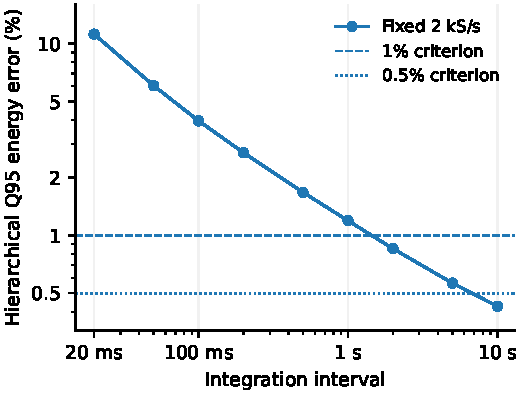
\includegraphics[width=\columnwidth]{jetson_rate_duration.pdf}
\caption{Jetson fixed-rate energy reconstruction. Each point is the largest hierarchical Q95 error across six workloads and two acquisition paths at 2 kS/s. Markers are tested durations; connecting segments guide the eye, not a guarantee at untested intervals. The 59 executions supply the physical repeats.}
\label{fig:jetson-energy}
\end{figure}

This duration effect is not a statement that fewer samples always suffice. A long integral can average positive and negative deviations over repeated fluctuations, whereas short windows are more exposed to alignment with their local structure. The reference experiment keeps the execution fixed so this numerical effect is not confused with startup, completed work or changes in device state. It therefore answers whether the sampled representation preserves \emph{a specified integral}, not whether a requested benchmark duration is representative of deployment.

\subsection{A Passing Operating Point Is Not a Universal Minimum}
Table~\ref{tab:reference} reports all nine durations together with the persistent decisions from~\eqref{eq:persistent}. For a 1\% tolerance, the tested persistent minimum is 160 kS/s at 20 ms, 80 kS/s at 100 ms and 16 kS/s at 1 s. Longer windows lower the requirement further: 1.2 kS/s at 5 s and 680 S/s at 10 s. The stricter 0.5\% objective remains unattained at the two shortest durations within the evaluated grid.

\begin{table}[t]
\caption{Native Jetson energy reconstruction over all nine durations. Error is the hierarchical envelope at a fixed 2 kS/s. The two $f_{\min}$ columns require that rate and every higher eligible tested rate to pass. A dash means not attained up to 160 kS/s, not an inferred requirement beyond it.}
\label{tab:reference}
\centering\footnotesize
\begin{tabular}{@{}lrrr@{}}
\toprule
Interval & Error (\%) & $f_{\min,1\%}$ (S/s) & $f_{\min,0.5\%}$ (S/s) \\
\midrule
20 ms & 11.23 & 160 k & --- \\
50 ms & 6.05 & 80 k & --- \\
100 ms & 3.96 & 80 k & 160 k \\
200 ms & 2.70 & 80 k & 80 k \\
500 ms & 1.68 & 16 k & 80 k \\
1 s & 1.19 & 16 k & 80 k \\
2 s & 0.85 & 16 k & 16 k \\
5 s & 0.56 & 1.2 k & 16 k \\
10 s & 0.43 & 680 & 16 k \\
\bottomrule
\end{tabular}

\end{table}

The 2-s result explains why both kinds of decision matter. Fixed 2 kS/s passes with an error of about 0.85\%, yet the tested 9.4-kS/s point rises just above 1\%. The persistent 1\% minimum is consequently 16 kS/s, not 2 kS/s. At 10 s, fixed 2 kS/s likewise passes 0.5\%, while that tolerance's persistent minimum remains 16 kS/s. Increasing a rate need not monotonically improve every finite-grid reconstruction because the sampled locations also change.

For an instrument operating at a known fixed rate, the corresponding pointwise test answers the practical question. For a recommendation expressed as ``at least this rate'', the persistent rule retains the higher-rate failures that the wording would otherwise hide. Both results are meaningful; neither permits interpolation of an unmeasured threshold or unconditional transfer to another analogue front end.

\subsection{Long-Window Energy Provides a Different Operating Point}
The separate GEMM-FP16 cohort extends the duration perspective to nominal 104-s intervals. All 15 recordings are retained, with 64 offsets each at the three evaluated rates. Its pooled Q95 error is about $\FPFifty\%$ at 50 S/s, about 0.49\% at 85 S/s and about 0.09\% at 2 kS/s. This is a different cohort and aggregation from the six-workload hierarchy, but it makes the long-window consequence tangible: a much sparser grid can still preserve an execution's integrated energy.

The percentile should not be read as a bound on every case. At 50 S/s, individual errors exceed 1\%; at 85 S/s, all 960 evaluated recording/offset cases remain below 1\%. Those are separate operational choices: tolerating a small upper tail of observed errors versus requiring every evaluated case to pass. Figure~\ref{fig:energy-spectrum}(a) retains both summaries rather than calling the percentile an absolute accuracy specification.

The low-rate result applies to integration over the retained long interval. It does not establish the performance of a physical 50-S/s instrument, adequate timing of individual inferences, or preservation of the fluctuations within the interval. The next question tests precisely what the successful energy integral leaves unresolved.

\section{RQ2: Preserving Energy Does Not Preserve Fluctuations}
\label{sec:dynamics}
\subsection{The Same Recordings Support Different Measurement Objectives}
The FP16 energy result and its spectrum describe the same experimental workload but very different outputs. At 2 kS/s, only about 4\% of the measured positive excess fluctuation variance lies below Nyquist, despite the small long-window energy error. The average can therefore be well represented while most recorded fluctuation variance lies outside the proposed observation band. A small integration error is not evidence of a faithful temporal description.

\begin{figure*}[t]
\centering
\begin{minipage}[t]{.48\textwidth}\centering
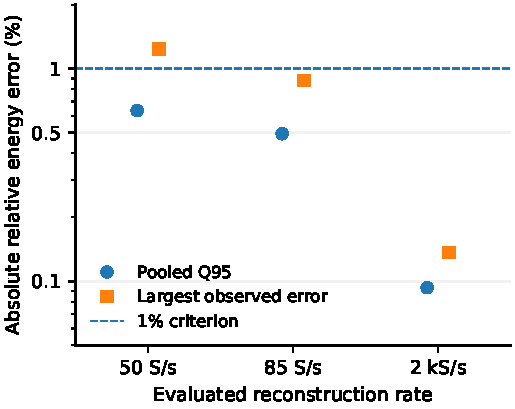
\includegraphics[width=\linewidth]{fp16_energy_objective.pdf}\\[-1mm]
\small (a) Energy over a nominal 104-s interval
\end{minipage}\hfill
\begin{minipage}[t]{.48\textwidth}\centering
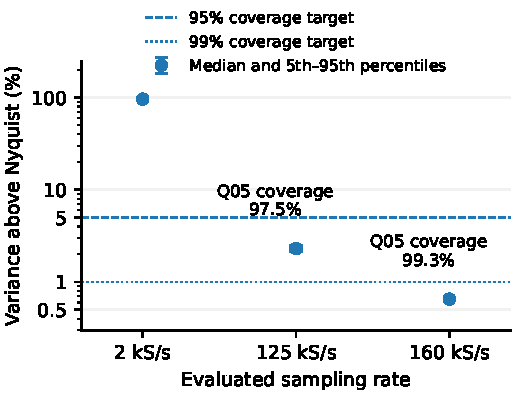
\includegraphics[width=\linewidth]{fp16_fluctuation_coverage.pdf}\\[-1mm]
\small (b) Positive-excess fluctuation coverage
\end{minipage}
\caption{Different objectives in the all-15-recording FP16 cohort. (a) Pooled Q95 and the largest observed energy error at three evaluated reconstruction rates, with 64 offsets per recording. (b) Measured variance above the candidate Nyquist frequency; markers show medians and bars empirical fifth--95th percentiles from matched active/idle intervals. The horizontal limits correspond to 95\% and 99\% coverage. The rate sets differ because the objectives differ; neither panel implies an untested minimum.}
\label{fig:energy-spectrum}
\end{figure*}

At the evaluated 125 and 160 kS/s rates, the lower empirical coverage percentiles are about 97.5\% and 99.3\%, respectively. Those points meet the 95\% and 99\% objectives defined in Section~\ref{sec:spectral-method}. Their practical role is not to replace the low-rate energy result: they answer how much \emph{measured fluctuation variance} remains below Nyquist. The useful rates for these two questions differ by orders of magnitude.

The distinction also clarifies the denominator of a spectral claim. Positive excess subtracts an idle spectrum, clips negative differences and retains the acquisition response. Matching active and idle segment lengths and testing alternative idle portions leave the FP16 coverage decisions intact, but they do not turn positive excess into a noise-free physical workload spectrum. The result is a robust observation for the declared estimator, rather than a universal analogue-bandwidth specification.

For energy benchmarking, the implication is to select a rate for the integral and interval actually reported. For timing individual bursts or analysing fast power structure, that success is insufficient: the spectrum and acquisition path must be examined separately. Sampling more quickly can help the second task even when it changes the first task very little.

\subsection{Agreement Within a Common Band Is a Different Result}
The paired Jetson scopes make the acquisition dependence visible independently of a platform comparison. Their positive-excess cumulative power spectra differ by up to about 31 percentage points over the full recorded band. When each curve is normalised within 0--77 kHz, the largest differences fall to approximately 3 points (Fig.~\ref{fig:cdf}). The paths give much closer descriptions of how their measured low-band variance is distributed than of the fraction in the full band.

\begin{figure}[t]
\centering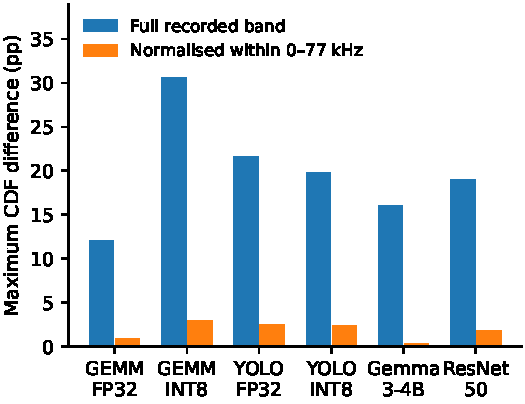
\includegraphics[width=\columnwidth]{native_cdf.pdf}
\caption{Acquisition-path dependence of native Jetson power spectra. Bars show the maximum Tektronix/PicoScope cumulative-distribution difference across frequency. Independent normalisation within 0--77 kHz changes the denominator; closer conditional shape is not proof of equal total variance or a measured transfer function.}
\label{fig:cdf}
\end{figure}

Conditional normalisation changes the denominator, so the improved agreement is not recovery of a true spectrum. The two paths can still measure different total variance. Their closer low-band shape is therefore useful only with its stated acquisition and normalisation conditions.

\subsection{Hailo Makes the Spectral Question Workload-Specific}
Hailo GEMM and YOLO have similar long-window card-input mean powers in their duration studies, but their spectral tails differ substantially. Figure~\ref{fig:hailo-spectra} uses separate 10-s active prefixes from 15 recordings of each workload. For GEMM, the median frequency enclosing 99\% of active variance is about 73 kHz, falling to about 27 kHz for positive active-minus-idle variance. For YOLO, the corresponding change is smaller, from about 105 to 95 kHz.

\begin{figure}[t]
\centering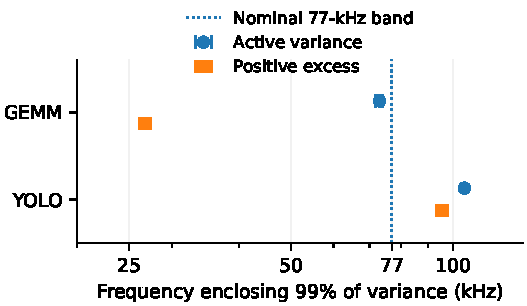
\includegraphics[width=\columnwidth]{hailo_spectral_tail.pdf}
\caption{Hailo spectral tails: median $f_{99}$ for active and positive-excess power variance, with empirical fifth--95th percentile ranges across 15 recordings per workload. The nominal current-path bandwidth is contextual, not a hard cutoff. Idle subtraction changes the GEMM tail much more than the YOLO tail; neither is an energy-rate threshold.}
\label{fig:hailo-spectra}
\end{figure}

The comparison has two implications. First, reporting a single bandwidth for ``Hailo inference'' would obscure workload-specific recorded dynamics. Second, the estimator matters: including the idle contribution changes GEMM's upper-tail description considerably. Positive excess is useful for separating an operational baseline from additional recorded variance, but clipping a difference spectrum is not a proof that noise has been removed. We therefore state the active/idle treatment rather than presenting $f_{99}$ as a hardware property.

The 95-kHz YOLO tail also illustrates why the nominal 77-kHz analogue bandwidth is not a brick-wall cutoff. Measured content can remain above that nominal value, while the acquisition response still shapes the signal. These observations do not identify layers, frames or compiler operations as peak causes; the datasets do not provide the synchronous markers needed for that attribution.


The combined spectral evidence therefore broadens rather than replaces the energy argument. Jetson demonstrates the separation between integrals and fluctuations, the paired scopes demonstrate acquisition-path dependence, and Hailo demonstrates workload dependence on another accelerator class. None supplies a Hailo or discrete-GPU energy-rate threshold without a corresponding unchanged-endpoint reconstruction. What can be carried to another platform is the measurement procedure; a numerical threshold requires its own evidence.

\section{RQ3: Agreement Depends on What and When We Measure}
\label{sec:meters}

\subsection{A Complete Jetson Deployment Check}
The reconstruction and spectrum determine what to test; deployed instruments still have to agree under the actual benchmark protocol. Figure~\ref{fig:jetson-meters} presents the Jetson comparison at a 300-s request. Each of seven workloads contributes 15 executions observed by PicoScope and three comparators. The resulting 315 comparator pairs represent 105 physical executions, not 315 independent benchmarks. Their medians are computed after pairing as in~\eqref{eq:paired}.

\begin{figure}[t]
\centering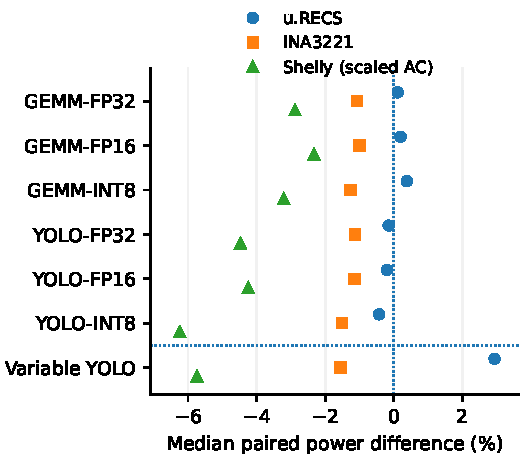
\includegraphics[width=\columnwidth]{jetson_deployed_meters.pdf}
\caption{Jetson deployed-meter comparison at a 300-s request. Markers show the medians of individual mean-power differences from PicoScope, with 15 matched executions per workload. Variable YOLO is separated from the six continuous workloads. Per-run windows and recorded scaling are retained; full pair percentiles are in the numerical artefact.}
\label{fig:jetson-meters}
\end{figure}

For the six continuous GEMM and YOLO workloads, every \urecs{} median difference is within $\pm0.5\%$. This is useful evidence for the deployed embedded 2-kS/s path in those long, continuous measurements. It complements the fixed-endpoint numerical test without converting the reconstruction criterion into an absolute instrument-accuracy claim. Individual differences and other activity patterns can still behave differently.

INA3221 input telemetry is about 1.0--1.5\% lower than PicoScope across those continuous workloads. Empirically scaled Shelly observations are about 2--6\% lower and more workload-dependent. A repeatable signed displacement is not removed simply by averaging more repeats. Conversely, the AC comparison includes its specific transformation and electrical domain; it is not an isolated specification of the plug meter.

Variable YOLO provides the critical contrast. The \urecs{} median difference rises to approximately +2.9\% without a change in nominal acquisition rate. The data do not identify the mechanism, because the devices retain their own intervals and responses. They do establish why continuous-load agreement is not sufficient evidence for intermittent operation. This complete Jetson check is the starting point for the attached-card experiment, not an assumed accuracy specification transferred to it.

\subsection{Close DC Agreement Carries Over to the Hailo Card}
The 300-s comparison first asks whether the embedded sensing path can reproduce the long-window external observation at the selected card input. It can do so closely in the tested Hailo workloads. Median \urecs{}--PicoScope power differences are about +0.40\% for GEMM, +0.45\% for YOLO and +0.19\% for variable YOLO (Fig.~\ref{fig:meters}). These are paired results from 15 executions per workload, not a comparison of unrelated benchmark averages.

\begin{figure*}[t]
\centering
\begin{minipage}[t]{.48\textwidth}\centering
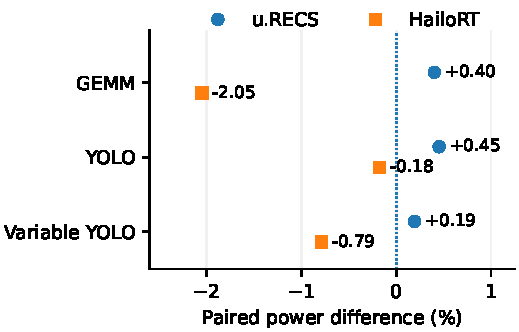
\includegraphics[width=\linewidth]{hailo_dc_telemetry.pdf}\\[-1mm]
\small (a) Embedded sensing and vendor telemetry
\end{minipage}\hfill
\begin{minipage}[t]{.48\textwidth}\centering
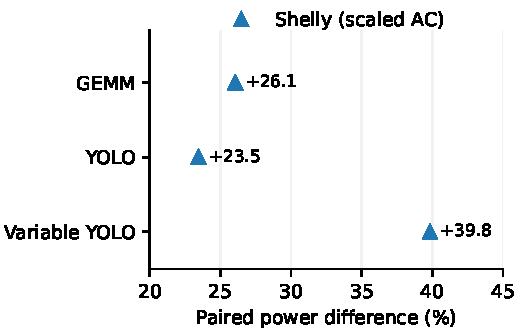
\includegraphics[width=\linewidth]{hailo_ac_context.pdf}\\[-1mm]
\small (b) Scaled observation at the AC boundary
\end{minipage}
\caption{Hailo at a 300-s request. Markers are medians of per-execution mean-power differences from PicoScope, with 15 paired executions per workload. The panels use different horizontal ranges to keep the DC/telemetry differences readable. Shelly is an empirically scaled AC observation, not another card-input sensor. Each path retains its own integration interval; all pair values and percentiles accompany the figure.}
\label{fig:meters}
\end{figure*}

HailoRT is also repeatable within workloads, but its central agreement is not constant across them: about $-2.05\%$ for GEMM, $-0.18\%$ for YOLO and $-0.79\%$ for variable YOLO. Narrow repeated observations do not by themselves remove this workload dependence. The result supports long-window, workload-specific use of the interface; it does not establish a universal telemetry correction or its response to individual short events.

The two platforms therefore share close embedded/external agreement during the tested long continuous workloads, but their variable-activity results differ. The smaller Hailo variable-YOLO difference does not establish a superior architecture: its deployment and explicitly retained interval differ from the Jetson case. The appropriate conclusion is workload-specific validation at each boundary, not one transferred correction factor.

\subsection{A Wider Electrical Boundary Changes the Interpretation}
The scaled Shelly observations in Fig.~\ref{fig:meters}(b) are roughly 23--40\% above the Hailo card-input readings. This is a larger difference than between the DC paths, but it is not evidence that the plug meter is intrinsically inaccurate. It observes the supplied AC arrangement and retains an empirical transformation; card input does not include conversion or other connected loads. Those quantities should be distinguished before interpreting the difference.

The direction is itself informative. In the continuous Jetson comparisons, the scaled AC estimates lie about 2--6\% \emph{below} PicoScope, whereas they lie above card input for all three Hailo workloads. A universal statement such as ``AC measurements are higher'' or a single cross-platform scaling correction would not describe these results. The combined effects of measurement boundary, applied transformation and interval must remain part of the reported quantity.

Likewise, the 40\% relative difference for variable Hailo activity cannot be relabelled as a 40\% host-energy share. A relative difference uses card-input power as its denominator, and the AC path need not contain a separately measured host. Quantifying component shares requires compatible, aligned component observations. The present comparison establishes the practical consequence of distinct boundaries, not a measured decomposition of them.

\subsection{Mean-Power Agreement Can Hide an Interval Mismatch}
A 300-s average is only one operating point. Applying the same pairing to all ten duration requests shows that HailoRT mean-power agreement changes most at the shortest requests. For continuous YOLO, its median difference moves from approximately $-3.3\%$ at 5 s to $-0.18\%$ at 300 s; GEMM changes from roughly $-3.8\%$ to $-2.1\%$. Variable YOLO appears comparatively stable when only mean power is inspected (Fig.~\ref{fig:intervals}(a)).

\begin{figure*}[t]
\centering
\begin{minipage}[t]{.48\textwidth}\centering
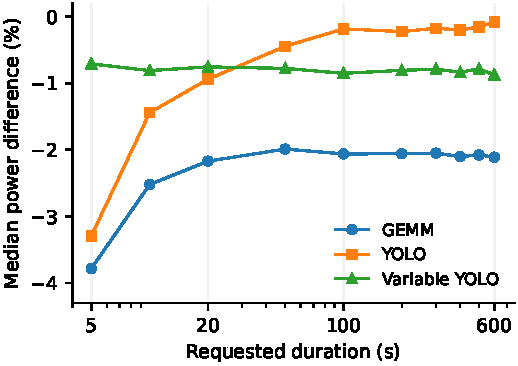
\includegraphics[width=\linewidth]{hailort_duration.pdf}\\[-1mm]
\small (a) HailoRT mean-power agreement by workload
\end{minipage}\hfill
\begin{minipage}[t]{.48\textwidth}\centering
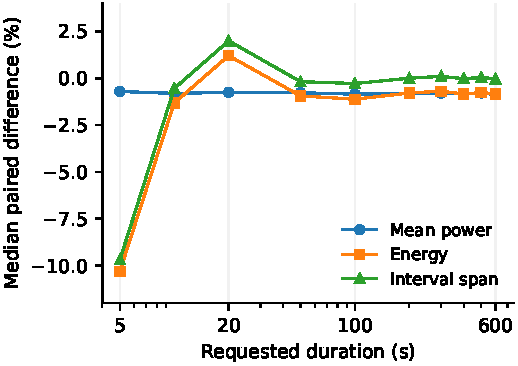
\includegraphics[width=\linewidth]{hailo_variable_intervals.pdf}\\[-1mm]
\small (b) Variable YOLO: power, energy and span
\end{minipage}
\caption{Duration-wise HailoRT--PicoScope pairing from the same stored measurement outputs, with 15 pairs at each request. Each point is the median of the individual relative differences. In (b), power agreement alone conceals a short-request interval difference. The retained explicit PicoScope interval for variable YOLO includes padding; these curves do not compare common physical endpoints or measure telemetry latency.}
\label{fig:intervals}
\end{figure*}

The energy comparison reveals why that apparent stability is incomplete. At a 5-s variable-YOLO request, the HailoRT median mean-power difference is only $\VariablePowerFive\%$, but the median energy difference is $\VariableEnergyFive\%$. Its median interval-span difference is $\VariableSpanFive\%$. The explicitly retained PicoScope interval is seven seconds because padding is included, whereas the telemetry interval is shorter. Equation~\eqref{eq:identity} links these quantities within every recorded pair. Agreement in mean power has not validated the energy interval.

At 300 s, the corresponding power and energy differences are both below 1\% in magnitude, and the relative span difference is small. A long-window agreement result can therefore coexist with a materially different short-request energy result. The conclusion is not that telemetry loses a proven fraction of the physical event: the retained endpoints differ, and no synchronised onset test is implied. It is that interval verification is necessary before an aggregate meter comparison can support an energy claim.

This distinction also clarifies what numerical resampling can and cannot fix. Increasing the density of samples inside an unchanged, shorter interval cannot supply energy outside that interval. Calibration and sample-rate selection remain useful, but they address different parts of the observed disagreement.

\section{RQ4: Validate the Execution as Well as the Meter}
\label{sec:protocol}
\subsection{A Short Benchmark Is Not Automatically Representative}

The interval in the numerical reconstruction is held fixed. A benchmark's requested duration, in contrast, can alter which execution phases contribute to its measured average. Figure~\ref{fig:duration} keeps the DC path fixed within each series and compares each actual $E/T$ with that workload's 600-s-request median. This asks whether a shorter execution gives a similar measured mean, not whether its samples reproduce an unchanged reference trace.

\begin{figure*}[t]
\centering
\begin{minipage}[t]{.48\textwidth}\centering
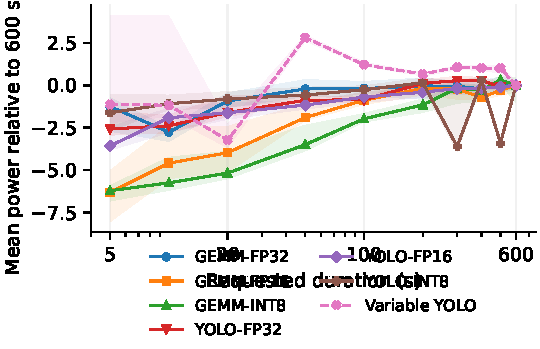
\includegraphics[width=\linewidth]{jetson_duration.pdf}\\[-1mm]
\small (a) Jetson
\end{minipage}\hfill
\begin{minipage}[t]{.48\textwidth}\centering
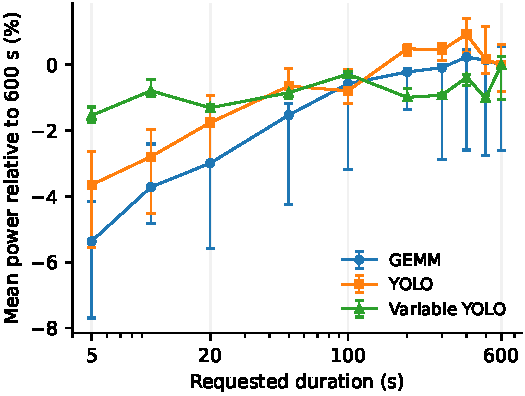
\includegraphics[width=\linewidth]{hailo_duration.pdf}\\[-1mm]
\small (b) Hailo
\end{minipage}
\caption{Duration dependence of per-run mean power $E/T$, relative to each workload's 600-s-request median. Markers or curves show group medians; shaded bands in (a) and bars in (b) show empirical fifth--95th percentiles, not confidence intervals. The actual recorded span defines $T$. Jetson uses available valid load intervals; each Hailo group contains 15 executions and variable YOLO retains its explicit padded interval.}
\label{fig:duration}
\end{figure*}

For Jetson GEMM-FP16, a 5-s request gives about 6.3\% less mean power than the 600-s group, while its median detected load span is only 3.0 s. This is not in conflict with accurate reconstruction over a specified two-second window: the shorter benchmark and the longer benchmark are different executions. Startup, activity fraction and operating state can differ before any integration error is considered. At a 100-s request, the six continuous Jetson medians are within 2\% of their respective 600-s values.

Hailo provides an analogous but not numerically identical duration dependence. Its 5-s GEMM and YOLO requests give about 5.4\% and 3.6\% less mean power than their own 600-s groups. By 100 s, their medians are within 0.8\%. Longer execution reduces the observed differences in these cohorts, but 600 s remains a comparison point rather than a demonstrated steady-state limit. The observations do not establish 100 s as a universal minimum benchmark duration.

Variable activity deserves its own interpretation. Hailo's recorded interval includes padding and internal pauses. Averaging over that interval describes the retained schedule, not only accelerator-active samples. Removing those portions after seeing the result would change the quantity rather than improve its accuracy. An activity-only mean and a schedule-level energy can both be meaningful, but their definitions must precede their comparison.

\subsection{Repeatability Is a Prerequisite for a Rate Sweep}
Direct rate sweeps compare different physical executions. Their variation includes the executed work, acquisition order, starting conditions and interval selection, in addition to the configured rate. Table~\ref{tab:repeatability} retains all eight Jetson and four Hailo series under the same definitions; no series is selected merely for having a favourable trend. Hailo makes the importance of execution repeatability particularly visible. Continuous GEMM and YOLO are comparatively repeatable; variable activity is more dispersed, and the LLM-labelled series reaches a within-rate energy CV of about $\HailoLLMCV\%$.

\begin{table}[t]
\caption{Direct Jetson and Hailo sweeps. Each series has 27 rate groups except Jetson YOLO-FP32, which has 26. ``Max. shift'' compares a rate-group energy mean with the equally weighted mean of rate-group means. All finite results are retained; three LLM intervals are missing. These are between-execution statistics, not same-trace sampling errors.}
\label{tab:repeatability}
\centering\footnotesize\begin{tabular}{@{}lrrr@{}}
\toprule
Workload & Runs & Max. CV (\%) & Max. shift (\%) \\
\midrule
\multicolumn{4}{l}{\textit{Jetson}} \\
GEMM-FP32 & 405 & 0.37 & 0.40 \\
GEMM-FP16 & 405 & 0.73 & 2.08 \\
GEMM-INT8 & 405 & 0.63 & 1.69 \\
YOLO-FP32 & 390 & 0.41 & 0.89 \\
YOLO-FP16 & 405 & 0.44 & 0.25 \\
YOLO-INT8 & 405 & 0.73 & 0.31 \\
Variable YOLO & 405 & 0.49 & 0.56 \\
Gemma3-12B & 405 & 0.58 & 1.66 \\
\midrule
\multicolumn{4}{l}{\textit{Hailo}} \\
GEMM & 405 & 0.68 & 1.48 \\
YOLO & 405 & 1.01 & 1.20 \\
Variable YOLO & 405 & 9.45 & 6.74 \\
LLM & 402 & 46.06 & 24.30 \\
\bottomrule
\end{tabular}

\end{table}

The largest LLM group displacement is about $\HailoLLMShift\%$. Neither that displacement nor the three unavailable intervals can be explained simply by asking for a faster meter. They first require an account of execution and valid interval formation. Conversely, the small within-rate CVs of the continuous workloads do not prove that different rate groups share identical conditions. On Jetson, GEMM-FP16 combines a maximum within-rate CV below 0.8\% with a largest group displacement of about 2.1\%. Repeatability within a group and comparability between groups are separate checks.

A fixed interior-window analysis of 225 Jetson recordings retains some of the between-rate differences after excluding the detected outer edges~\cite{energyResults2026}. This rules out attributing the entire observation to one envelope boundary, but it still compares separate executions. A more controlled acquisition sequence is therefore needed before assigning a change to the configured rate.

\subsection{Order Control Narrows the Rate-Associated Difference}
The complementary GEMM-FP16 control fixes the engine, 250 completed TensorRT queries, spin-wait option and 120-s process-end-to-next-start pause. With $A=2$ kS/s and $B=5$ MS/s, the two session orders are ABBAAB and BAABBA. Every sequence position is observed once at each rate across the two sessions. All twelve runs are retained.

We fit an additive model with a rate indicator, a session term and categorical sequence-position effects. With eight independent design columns and twelve observations, it has four residual degrees of freedom. The rate estimate and its two-sided 95\% $t$ interval are expressed relative to the observed 2-kS/s outcome mean. The model does not fit rate-by-session interactions or supply an absolute measurement uncertainty.

\begin{table}[t]
\caption{Fixed-work FP16 rate control: adjusted 5-MS/s-minus-2-kS/s changes. The two final columns give the lower and upper model-based 95\% bounds. Six executions are measured at each rate; the intervals are not equivalence limits.}
\label{tab:control}
\centering\footnotesize\begin{tabular}{@{}lrrr@{}}
\toprule
Quantity & Change (\%) & \multicolumn{2}{c}{95\% interval (\%)} \\
\midrule
External DC power & -0.06 & -0.18 & +0.06 \\
Input telemetry & +0.01 & -0.07 & +0.09 \\
250-query runtime & -0.03 & -0.17 & +0.11 \\
\bottomrule
\end{tabular}

\end{table}

The adjusted external load-power difference is about $-0.06\%$, with bounds of approximately $-0.18\%$ and $+0.06\%$ (Table~\ref{tab:control}). Input telemetry and query time likewise resolve no clear rate-associated change under this model. This is compatible with low reconstruction error at the intended embedded rate, but it is not proof that all rates or workloads are equivalent. The controlled outcome is deliberately narrower: the multi-percent difference seen between some separate groups is not a stable rate-associated effect in this fixed-work, balanced comparison.

\subsection{The Starting State Can Change While the Rate Stays Fixed}
A separate GEMM-FP32 diagnostic reverses the question. Acquisition remains at 2 kS/s in one continuous stream, while the process pause changes between 20 and 120 s. One conditioning execution is excluded by design; six scored executions follow the pause sequence 20, 120, 120, 20, 20, 120 s, with 100 completed TensorRT queries each~\cite{pauseEvidence2026}.

\begin{figure}[t]
\centering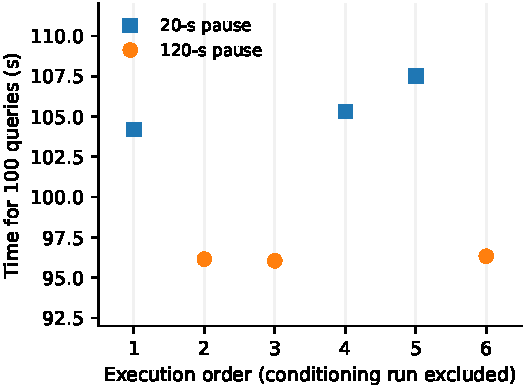
\includegraphics[width=\columnwidth]{pause_runtime.pdf}
\caption{Fixed-rate FP32 pause diagnostic in execution order. Every scored run completes 100 queries; one preceding conditioning run is excluded. All long-pause runs are faster in this sequence. Three repeats per condition in one session support a protocol diagnostic, not an isolated causal temperature or throttling claim.}
\label{fig:pause}
\end{figure}

Median runtime decreases from approximately 105.3 s after short pauses to 96.2 s after long pauses, or $\PauseReduction\%$ (Fig.~\ref{fig:pause}). Median pre-start GPU temperatures are about 74 and 59~$^{\circ}$C, respectively. These observations come from timing and platform logs, so an external power-window choice cannot create the runtime change. The experiment demonstrates that execution state matters even when the meter's configured rate does not change.

It does not isolate a temperature mechanism. The sampled GPU-frequency readout remains unchanged, while thermal history and preceding work are coupled in this small sequential study. We therefore use timing and temperature as evidence for documenting the starting state, not as proof of a particular throttling threshold. The diagnostic's external power calibration is not independently validated for absolute Jetson energy, and waiting energy is outside its activity interval. No claim that longer waits minimise total schedule energy follows from the runtime result.

The two controls complement rather than replace one another. Balanced acquisition narrows a rate-associated estimate; fixed-rate pauses demonstrate an independent execution dependency. Together they explain why a deployed energy benchmark needs both a validated observation and a repeatable protocol.

\section{Practical Implications and Scope}
\subsection{Validate a Measurement Configuration, Not a Sampling Number}
The results support a staged decision. Start with the electrical boundary and intended quantity: interval energy, activity mean power, schedule energy or fluctuation structure. Choose the endpoints and keep startup, transfers and internal pauses either explicitly inside or outside them. A reference recording can then test candidate sampling grids for that integral; a separate spectral criterion is needed when temporal detail is itself the output.

Next, deploy the selected configuration and test it with the actual workload. Pair repeated observations before aggregation, and inspect energy, mean power and span together. The Hailo variable-activity example shows why this is more informative than a single power ratio: a small power difference can coexist with a much larger energy difference when the intervals differ. Repeated long-window agreement is useful evidence for that operating point, not a substitute for testing a shorter interval.

Finally, validate the execution protocol. Specify completed work where it is known, request semantics where it is not, starting conditions and inter-execution pauses. Use balanced or randomised acquisition order when estimating rate-associated effects. The 600-s group can be a practical within-series comparator without being called a universal steady state, and a six-run pause test can expose a confound without supplying a general thermal model.

\subsection{What the Cross-Platform Comparison Establishes}
The Hailo results extend the Jetson evidence in a concrete but bounded way. Long-window embedded/external agreement also occurs at an attached card input; vendor agreement remains workload-dependent; the scaled AC difference changes direction between setups; and short-request energy and mean-power agreement can diverge. Hailo spectra add a separate warning against transferring a fluctuation requirement solely from a platform label.

These observations do not constitute an accelerator-efficiency ranking. The module and card boundaries include different components, and identical workload names do not establish identical completed inference work. A quantitative host fraction requires aligned component observations, not subtraction of an unexplained AC/DC difference. Similarly, the presented native Jetson error envelope does not certify a Hailo or discrete-GPU energy rate without the corresponding same-trace test.

The duration-wise HailoRT comparison is also intentionally distinct from dynamic sensor validation. Its own intervals are part of the observations. It does not measure internal update cadence, onset delay or loss of a synchronised event. Those properties require timing evidence beyond paired aggregate outputs. This limit does not invalidate the aggregate comparison; it specifies which measurement decision the comparison can support.

\subsection{Traceability of the Argument and Its Limits}

The statistical and electrical limits remain separate. Empirical pair percentiles describe recorded repeats; hierarchical quantiles describe reconstruction cases and recordings; PSD area describes measured fluctuation variance. None is a complete dynamic-power uncertainty budget. Current-model extrapolation, the workload-derived scope correction and setup-specific scaling remain part of the interpretation. Nor does the nominal 77-kHz front end guarantee anti-alias protection at 2 kS/s.

The source package provides full-precision pair values, interval policies, calibration information, spectral and reconstruction summaries, and generators for every numerical figure and table. Evidence is pinned to a repository commit~\cite{energyResults2026,pauseEvidence2026}; the preceding Jetson study is cited at its fixed author-manuscript version~\cite{mika2026workshopdraft}. Regeneration from stored outcomes is distinct from raw-waveform reconstruction or PSD re-estimation, which require the original recordings and matching acquisition settings.

\section{Conclusion}
A useful energy measurement requires more than a sufficiently high sampling rate. Across six Jetson workloads, fixed 2 kS/s meets the empirical 1\% energy criterion at the tested 2-, 5- and 10-s intervals, while a 100-ms interval requires a persistent 80-kS/s minimum. The separate FP16 study shows why long energy integration and fluctuation analysis need markedly different rates. The Hailo extension shows why the next decision is about the deployed observation: electrical boundary, actual interval and workload determine what apparent meter agreement means.

Embedded sensing agrees closely with external DC acquisition during the tested long continuous workloads, while vendor and AC comparisons remain specific to their domains and transformations. Duration-wise Hailo pairing makes the distinction tangible: short-request mean-power agreement can conceal a much larger energy difference when the retained spans differ. Spectral characterisation and fixed-rate protocol controls add complementary evidence that neither a stable average nor a faster meter alone establishes representative execution or temporal fidelity.

The practical recommendation is therefore to validate the measurement configuration as a whole: define the quantity and boundary, test the rate against its interval, compare energy together with power and span, and verify the execution conditions. This supports repeatable, workload-specific energy assessment without turning one successful operating point into a universal sampling rule or meter-accuracy ranking.

\bibliographystyle{IEEEtran}
\bibliography{references}
\end{document}
